\documentclass[../main.tex]{subfiles}
\graphicspath{
    {"../img/"}
    {"img/"}
}

\begin{document}
    \subsection{Równania różniczkowe}
    Interesuje nas następująca sytuacja:
        $
        \frac{dx}{dt} = f(t,x) \\
        x(t_0)= x_0\\
        x(1): [a,b]\to\mathbb{R}\\
        f: [a,b]\times \mathbb{R}^n\to\mathbb{R}^n
        $
        \begin{przyklad}
            \begin{align*}
                \frac{dx}{dt} = -kx(t)\\
                x(t) = c e^{-kt}
            .\end{align*}
        \end{przyklad}
        Pytanie: czy to, że równanie jest pierwszego rzędu bardzo nam przeszkadza?\\
        \begin{przyklad}
            $\ddot{x} + \omega^2 x = 0\\
            \dot{x} = p\\
            \dot{p} = \ddot{x} = -\omega^2 x\\
            \frac{d}{dt} \underbrace{\begin{bmatrix} x\\p \end{bmatrix}}_{\frac{d}{dt}x} =
            \underbrace{\begin{bmatrix} 0&1\\ -\omega^2&0 \end{bmatrix}
            \begin{bmatrix} x\\p \end{bmatrix}}_{f(x,t)}
            $

        \end{przyklad}
        \begin{definicja}
            Niech $I\subset \mathbb{R}, \mathcal{O}\subset \mathbb{R}^n$ \\
            $f: I\times\mathbb{R}^n \to \mathcal{O}$ taka, że $t\in I, x\in \mathbb{R}^n, f(t,x) \to f(t,x)$\\
            Mówimy, że $f$ spełnia warunek Lipschitza, jeżeli
            \[
                \underset{L>0}{\exists}. \underset{t\in I}{\forall}. \underset{x,x'\in \mathcal{O}}{\forall}. \Vert f(t,x) - f(t,x')  \Vert \leq L \Vert x - x' \Vert
            .\]
        \end{definicja}
        \begin{uwaga}
            Znane $t,x$ nie występują w warunku Lipschitza na równych prawach
        \end{uwaga}
        \begin{pytanie}
            Czy jeżeli \[
                f:\mathcal{O}\to\mathcal{O}\text{ takie, że } \underset{L>0}{\exists}
            .\] że \[
            \underset{x,x'}{\forall}  \Vert f(x) - f(x') \Vert \leq L \Vert x - x' \Vert
            .\] to czy $f $ jest ciągła?
        \end{pytanie}
        \begin{tw}
            Niech $[a,b] \subset \mathbb{R}, \mathcal{O}\subset\mathbb{R}^n, \mathcal{O}$ - domknięty i $f:[a,b]\times\mathcal{O}\to\mathcal{O}$ takie, że $f$ - ciągła na $[a,b]\times\mathcal{O}$ oraz $f$ spełnia warunek Lipschitza na $\mathcal{O}$, to znaczy:
            \[
                \underset{L>0}{\exists}. \underset{t\in[a,b]}{\forall}. \underset{x,x'\in\mathcal{O}}{\forall} \Vert f(t,x) - f(t,x') \Vert \leq L \Vert x-x' \Vert
            .\] Wówczas \[
            \underset{t_0\in[a,b]}{\forall} . \underset{x_0\in\mathcal{O}}{\forall} . \underset{\varepsilon>0}{\exists} \text{, że dla } t\in ]t_0-\varepsilon, t_0+\varepsilon[
            \]
            równanie ma jednoznaczne rozwiązania, które są ciągłe ze względu na $x_0$
            \begin{equation}
            \begin{cases}\label{eq:eq21}
                \frac{dx}{dt} = f(t,x)\\
                x(t_0) = x_0
            \end{cases}
            \end{equation}
        \end{tw}
        \begin{uwaga}
            Problem \ref{eq:eq21} nazywamy problemem Cauchy.\\
            Ciągłość $f$ na $[a,b]\times\mathcal{O}$ jest mocniejszym warunkiem niż Lipschytzowalność na $\mathcal{O}$
        \end{uwaga}
        \begin{figure}[h]
            \centering
            \includegraphics[width=0.8\textwidth]{fig_27}
            \caption{}
            \label{fig:fig_27}
        \end{figure}
        \begin{dowod}
            Skoro $f$ - ciągła na $[a,b]\times\mathcal{O}$, to znaczy, że $f$ jest ograniczona, czyli
            \[
                \underset{M>0}{\exists} . \underset{y_1>0}{\exists}. \underset{y_2>0}{\exists},\quad \Vert f(t,x) \Vert \leq M
            .\]
            $t\in K(t_0,y_1), x\in K(x_0,y_2)$.\\
            Zauważmy, że problem \ref{eq:eq21} możemy zapisać jako
            \begin{equation}\label{eq:eq22}
                x(t) = x_0 + \int_{t_0}^t f(s,x(s)) ds
            \end{equation}
            Czyli, jeżeli znajdziemy $x(t)$ takie, co spełnia \ref{eq:eq22}, to raslkdj problem \ref{eq:eq21}.\\
            Rozważmy odwzorowanie \[
                \underset{g\in a}{P(g)(t)} = x_0 + \int_{t_0}^t f(s,g(s))ds
            .\]
            \[
                A = \left\{ C: [t-r_1, t_0+r_1]\to \mathbb{R}^n \right\}\text{ funkcja ciągła na kuli o wartościach w }\mathbb{R}^n
            .\]
            \begin{figure}[h]
                \centering
                \includegraphics[width=0.8\textwidth]{fig_28}
                \caption{}
                \label{fig:fig_28}
            \end{figure}
            Co by było, gdyby $P$ miało punkt stały?
            Czyli $\underset{x(t)\in A}{\exists}$ takie, że $P(x(t)) = x(t)$\\
            Oznaczałoby to, że \[
                x(t) = -x_0 + \int_{t_0}^t f(s,x(s))ds
            .\] Co więcej, gdyby $P$ było zwężające, to z zasady Banacha wiemy, że punkt stały jest tylko jeden. Zatem, jeżeli znajdziemy podzbiór $A$ taki, że $P$ - zwężające, to udowodnimy jednoznaczność. Problem \ref{eq:eq22}\\
            Niech $E = \left\{ g\in \mathcal{C}([t_0-\varepsilon,t_0+\varepsilon],\mathbb{R}^n, \Vert g(t) - \overset{g_0(t)}{x_0} \Vert \underset{\text{ważne!}}{\leq} r_2 \right\} $, czyli \[
                g\in E \iff \underset{t_0-\varepsilon\leq t\leq t_0+\varepsilon}{sup} \Vert g(t) - x_0 \Vert \leq r_2
            .\] i \[
            g: [t_0-\varepsilon, t_0+\varepsilon]\to\mathbb{R}^n
            .\] i $g$ - ciągła.\\
            (domkniętość ze względu na zasdę Banacha $(x_0 \overset{\text{ozn}}{=} g_0(t) )$)

            Szukamy takiego $\varepsilon$, żeby:
            \begin{align}
                P(g)\in E \quad g\in E\label{eq:eq23}\\
                P\text{ - zwężająca na }E\label{eq:eq24}
            .\end{align}
            bo jeżeli \ref{eq:eq24} jest spełniona, to wiemy, że istnieje punkt stały.\\
            Jeżeli \ref{eq:eq23} jest spełniona, to wiemy, że punkt stały należy do  $E$\\
            Warunek \ref{eq:eq23}:
            $P(g)\in E$, czyli
            \[
                \underset{t_0-\varepsilon\leq t_0\leq t_0+\varepsilon}{sup} \Vert P(g(t)) - x_0 \Vert \leq r_2
            .\]
            czyli
            \[
                \underset{t_0-\varepsilon\leq t_0\leq t_0+\varepsilon}{sup} \Vert x_0 + \int_{t_0}^t f(s,g(s))ds - x_0 \Vert \leq \underset{t_0-\varepsilon\leq t_0\leq t_0+\varepsilon}{sup} \int_{t_0}^t \Vert f(s,g(s)) \Vert ds \leq
            .\]
            \[\underset{t_0-\varepsilon\leq t_0\leq t_0+\varepsilon}{sup} |t-t_0| M = \varepsilon M
            .\]
            Jeżeli chcemy aby $\varepsilon M \leq r_2$ \\
            to znaczy, że $\varepsilon \leq \frac{r_2}{M}$ \\
            i jednocześnie $\varepsilon\leq r_1$\\
            czyli aby warunek \ref{eq:eq23} był spełniony
            \[
                \varepsilon < min \left\{ \frac{r_2}{M}, r_1 \right\}
            .\]
            Warunek \ref{eq:eq24}. Chcemy aby $P$ było zwężające, czyli:
            \[
                \underset{g_1,g_2\in E}{\forall}  P(g_1) - P(g_2) \le q\Vert q_1-q_2 \Vert
            .\]
            Zatem:
            \[
                \Vert P(g_1) - P(g_2) \Vert  = \underset{t_0-\varepsilon\leq t_0\leq t_0+\varepsilon}{sup} \Vert x_0 + \int_{t_0}^t f(s,g_1(s))ds - (x_0 + \int_{t_0}^t f(s,g_2(s))ds \Vert =
            .\]
            \[
                \underset{t_0-\varepsilon\leq t_0\leq t_0+\varepsilon}{sup} \Vert \int_{t_0}^t f(s,g_1(s)) - f(s,g_2(s)) ds \Vert \le \underset{t_0-\varepsilon\leq t_0\leq t_0+\varepsilon}{sup} \int_{t_0}^t \Vert f(s,g_1(s)) - f(s,g_2(s)) \Vert ds \le
            .\]
            \[
                \underset{t_0-\varepsilon\leq t_0\leq t_0+\varepsilon}{sup} \int_{t_0}^t L \Vert g_1-g_2 \Vert = \varepsilon L  \underset{\substack{\in E\\ \Vert g_1 - g_2 \Vert < 2r_2}}{\Vert g_1 - g_2 \Vert}
            .\]
            Zatem, jeżeli $P$ ma być zwężające na $E$, to $\varepsilon L < 1$, czyli $\varepsilon< \frac{1}{L}$ i $g\in E$\\
            Zatem, aby istniało rozwiązanie jednoznaczne problemu \ref{eq:eq21} \[
                \varepsilon < min \left\{ \frac{r_2}{M}, r_1, \frac{1}{L} \right\} \quad\Box
            .\]
        \end{dowod}
        Do pełnego dowodu brakuje nam ciągłości rozwiązania ze względu na zmiany $x_0$

        Lemat:\\
        niech $A,X$ - przestrzenie metryczne, $P_a(x), a\in A, x\in X$ - odwzorowanie zwężające i ciągłe ze względu na $a\in A$\\
        Niech $\tilde x(a)$ taki, że $P(\tilde x(a)) = \tilde x(a)$. Zwężające, to znaczy, że \[
            \underset{a\in A}{\forall}. \underset{x,x'}{\forall}. \Vert P_a(x) - P_a(x') \Vert \le q \Vert x-x' \Vert
        .\] Wówczas funkcja $\tilde x(a)$ jest ciągła na $A$.
        \begin{uwaga}
            Odwzorowanie $P(g)$ wygląda tak:
            \[
                P(g(t)) = x_0 + \int_{t_0}^t f(s,g(s))ds
            .\] Więc rolę parametru $a$ pełnią $x_0,t_0$ i $P(g(t))$ jest ciągłe ze względu na $x_0$ i $t_0$.
        \end{uwaga}

\end{document}
